
% --------------------------------------------------------------
% This is all preamble stuff that you don't have to worry about.
% Head down to where it says "Start here"
% --------------------------------------------------------------

\documentclass[11pt]{article}

\usepackage{bera}
%\renewcommand{\familydefault}{\rmfamily}

\usepackage{graphicx,url}
\usepackage{proof}
\usepackage{framed}
\usepackage{etaremune}
\usepackage{hyperref}
\hypersetup{
    colorlinks=true,
    linkcolor=blue,
    filecolor=magenta,      
    urlcolor=blue,
    pdftitle={Overleaf Example},
    pdfpagemode=FullScreen,
    }
\usepackage[margin=1in]{geometry}
\usepackage{amsmath,amsthm,amssymb,amsfonts}
\usepackage{paralist}
\thispagestyle{empty}

% 1. To get version suitable for students to populate,
%    remove the contents of the \ignoreSoln{..body..}
%
% 2. To get a version suitable for generating PDF 
%    without solutions, remove the #1 below
%
% 3. To generate solutions, keep the #1 below
%
% 4. Assigned grader fills \ignoreSoln{..body..}
%    and also provides his/her feedback to student
%    and policy followed for point deduction
%    So design policy before grading begins.

\newcommand{\ignoreSoln}[1]{#1}   
%\newcommand{\ignoreModel}[1]{#1} 


\newcommand{\bigset}[2]{\big\{\;#1\;:\;#2\;\big\}}
\newcommand{\N}{\mathbb{N}}
\newcommand{\Z}{\mathbb{Z}}
\newcommand{\R}{\mathbb{R}}
\newcommand{\Np}{\mathbb{N^{+}}}

\newenvironment{theorem}[2][Theorem]{\begin{trivlist}
\item[\hskip \labelsep {\bfseries #1}\hskip \labelsep {\bfseries #2.}]}{\end{trivlist}}
\newenvironment{lemma}[2][Lemma]{\begin{trivlist}
\item[\hskip \labelsep {\bfseries #1}\hskip \labelsep {\bfseries #2.}]}{\end{trivlist}}
\newenvironment{exercise}[2][Exercise]{\begin{trivlist}
\item[\hskip \labelsep {\bfseries #1}\hskip \labelsep {\bfseries #2.}]}{\end{trivlist}}
\newenvironment{reflection}[2][Reflection]{\begin{trivlist}
\item[\hskip \labelsep {\bfseries #1}\hskip \labelsep {\bfseries #2.}]}{\end{trivlist}}
\newenvironment{proposition}[2][Proposition]{\begin{trivlist}
\item[\hskip \labelsep {\bfseries #1}\hskip \labelsep {\bfseries #2.}]}{\end{trivlist}}
\newenvironment{corollary}[2][Corollary]{\begin{trivlist}
\item[\hskip \labelsep {\bfseries #1}\hskip \labelsep {\bfseries #2.}]}{\end{trivlist}}

\DeclareMathSizes{14}{14}{14}{14}

\begin{document}

% --------------------------------------------------------------
%                         Start here
% --------------------------------------------------------------

%\renewcommand{\qedsymbol}{\filledbox}
\newlength{\minpagw}
\settowidth{\minpagw}{\hspace{40em}}

\begin{center}
\begin{large}
  CS 6110, Spring 2022, Assignment 6  \\
  Given 3/4/22 -- Due 3/15/22 by 11:59 pm via your Github 
  \ \\
%  \ \\  
    {  {\Large\bf NAME: Tripti Agarwal} \hfill {\Large\bf UNID: u1319433}\hspace{4cm} }
          \ \\
\end{large}

\end{center}


\begin{compactenum}

%- 1 ----------------------------------------------------------------
\item (40 points)

\begin{figure}[htp]
\begin{minipage}{\minpagw}
  \fbox{%
    \parbox{\linewidth}{%
      \begin{enumerate}
          \item (20 points)
          \begin{enumerate}
              \item (10 points)
              \begin{itemize}
                  \item \textbf{Logic 1.} Our universe U consists of two zero-ary predicate $r_0$ and $r_1$. There are two signatures a and b in the universe U. Each of the signatures (sets) have at least one relations defined on them named $R_0$ and $R_1$. The assertion says that $R_0$ implies $R_1$ implies $R_0$.  This means some element in a have a relation $r_1$ which implies another element in signature a having relation $r_2$, then $r_1$ implies the previous implication.
                  \item \textbf{Logic 2.} Some set U, S1 and S2 are sets that extends U. One-ary predicate p1 and two-ary predicate p2 are defined. p1 consists of elements that are in S1 and p2 consists of elements that either in S1 or in S2. The FOL EA says if at least one y in U and all x in U and predicate p2 in defined for these x and y then this implies that for all x and some y predicate p2 is true. The nEA is the negation of EA.
                  \item \textbf{Logic 3} The assertion EA is some y in U and all x in U such that p2 is true for all x and  f1(y), where f1 is 1-ary function i.i. one U, then this implies all x in U and some y in U p2(x, f1(y)) is true. The nEA is the negation of EA.
                  \item \textbf{Logic 4} Similar to logic 3 with the predicate consisting of all x in U and function f2 over some y in U. Here f2 is a 2-ary function.
                  \item \textbf{Logic 5} Signature a extends U. Sets S1, S2 and S3 are in U. At least one of the signatures of U has a property, where f is a function of U. Predicate P consists of x, y and z such that x is in S1, y is in S2 and z is in S3. Assertion EA, for all x in U and predicate P is true for elements a in S1, and x in S2 and S3. Also, all elements x, y and z in U such that P(x,yz) implies P(f(x), y , f(z)) then this implies that P(f(a), a, f(a)) is valid. nEA is negation of EA.
              \end{itemize}
              \item (10 points) \textbf{Logic4.als}
              The function f2 is a 2-ary function defined on set U such that each set maps to one U. This means set of U can either map to itself or to some other set of U. This can be seen in diagrams shown below:\\
              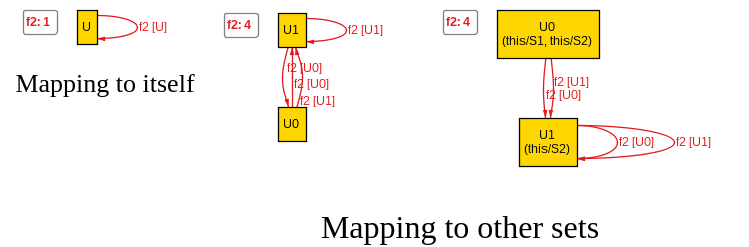
\includegraphics[width=5.0in]{q1.png}
          \end{enumerate}
      \end{enumerate}
    }%
  }%
\end{minipage}
\end{figure}

\begin{figure}[htp]
\begin{minipage}{\minpagw}
  \fbox{%
    \parbox{\linewidth}{%
      \begin{enumerate}
          \item (20 points) Above page
          \item (20 points) 
          \begin{enumerate}
              \item \textbf{Question 13(b)}
              The assertion is valid. The diagram below shows that no counter examples were found for EA where as counter examples are found when we check for nEA. The alloy code can be found on this 
              \href{https://github.com/tripti-agarwal/Formal-Method-verification/blob/main/Assignment6/Q1_b_1.als}{link}.
              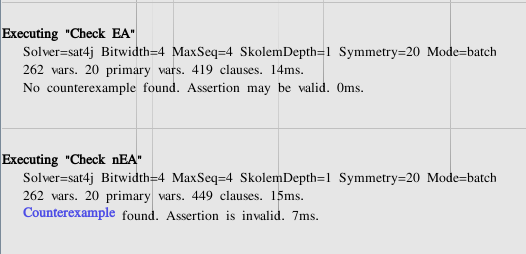
\includegraphics[width=5.0in]{q1_b_1.png}
              \item \textbf{Question 13(c)}
              The assertion is valid. The diagram below shows that no counter examples were found for EA where as counter examples are found when we check for nEA.  The alloy code can be found on this \href{https://github.com/tripti-agarwal/Formal-Method-verification/blob/main/Assignment6/Q1_b_2.als}{link}.
              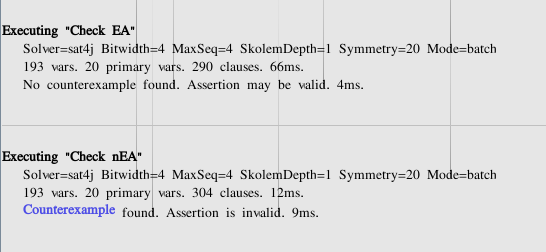
\includegraphics[width=5.0in]{q1_b_2.png}
          \end{enumerate}
        \end{enumerate}
}%
}%
\end{minipage}
\end{figure}
\newpage

%- 2 ----------------------------------------------------------------
\item (40 points)
  
\begin{minipage}{\minpagw}
  \fbox{%
    \parbox{\linewidth}{%
      \begin{enumerate}
          \item \textbf{20 points}
          \begin{enumerate}
              \item \textbf{(10 points) Mike Gordon's slides}
              \begin{itemize}
                  \item \textbf{Partial Correctness specification :} \{P\}C\{Q\} where P is the precondition and Q is the post-condition. This means that when C is executed satisfying P, then if the execution of C terminates, then the state in which the execution of C terminates satisfies Q.
                  \item \textbf{Total Correctness specification :} [P]C[Q]. If C is executed in a state satisfying P, then C definitely terminates, and after termination Q holds.
                  \item $\vdash$ S means that S has a proof. The statements that have a proof are called theorems.
                  \item $\frac{\vdash S_1,..., \vdash S_n}{\vdash S}$ says that conclusion $\vdash$ S may be deduced from $\vdash S_1,..., \vdash S_n$, which are the hypothesis of the rule.
                  \item \textbf{Hoare assignment axiom :} $\vdash$ \{P[E/V]\} V := E\{P\}. This means that the variable V after executing an assignment command V:= E equals the value of the expression E in the state before executing it. Formally, if a statement P is to be true after the assignment, then the statement obtained by substituting E for V in P must be true before executing it.
                  \item \textbf{Floyd assignment axiom} $\vdash$ \{P\} V := E \{$\exists$v. (V = E[v/V]) $\wedge$ P[v/V]\} where v is the new variable (i.e. doesn't equal V or occur in P or E).'
                  \item \textbf{Precondition strengthening} $\frac{\vdash P \Rightarrow P{^'}, ..., \vdash \{P{^'}\}C\{Q\}}{\VDASH \{P\} C \{Q\}s}$
                  \item \textbf{Post condition weakening} $\frac{\vdash \{P\}C\{Q{^'}\},..., \vdash Q{^'} \Rightarrow Q}{\vdash \{P\} C \{Q\}}$. The rules precondition strengthening and Post condition weakening are sometimes called the rules of consequences.
                  \item \textbf{Sequencing rule} This rules for the partial correctness specification for a sequence $C_1;C_2$ to be derived from specifications for $C_1$ and $C_2$. $\frac{\vdash \{P\}C_1\{Q\},...\vdash\{Q\}C_2\{R\}}{\vdash \{P\}C_1;C_2\{R\}}$
                  \item \textbf{Conditional/IF rule} $\frac{\vdash \{P \wedge S\} C_1 \{Q\},...,\vdash\{P\wedge \neg S\}C_2\{Q\}}{\vdash \{P\} \text{ IF S THEN } C_1 \text{ ELSE } C_2 \{Q\}}$
                  \item \textbf{WHILE-rule} $\frac{\vdash \{P \wedge S \} C \{P\}}{\vdash \{P\} \text{ WHILE S DO C } \{P \wedge \neg S\}}$
                  \item \textbf{FOR-rule} $\frac{\vdash \{P\} C \{P[V+1/V]\}}{\vdash \{P[E_1/V]\} \text{FOR V := $E_1$ UNTIL $E_2$ DO C }\{P[E_2+1/V]\}}$
              \end{itemize}

              
            \end{enumerate}
        \end{enumerate}
          
    }%
  }%
\end{minipage}
\newpage
\begin{minipage}{\minpagw}
  \fbox{%
    \parbox{\linewidth}{%
      \begin{enumerate}
          \item (20 points)
          \begin{enumerate}
              \item (10 points) Above page
              \item \textbf{(10 points) Dafny verifast installation}
              \begin{itemize}
                 \item \textbf{Verifast installation}
                 \begin{itemize}
                    \item Verifast can be installed by downloading a tar file from \url{https://github.com/verifast/verifast/releases}.
                     \item After this, follow the steps given below:
                    \begin{itemize}
                        \item tar xzf ~/Downloads/verifast-nightly.tar.gz
                        \item cd verifast-<TAB> \# Press Tab to autocomplete
                        \item bin/vfide examples/java/termination/Stack.jarsrc  \# Launch the VeriFast IDE with the specified example
                        \item ./test.sh \#  Run the test suite (verifies all examples)
                     \end{itemize}
                \end{itemize}
                \item \textbf{Dafny installation}
                    \begin{itemize}
                        \item  Installed Dafny in VS Code in ubuntu based system.
                        \item  VS Code provides a Dafny extension, which is just a one click install, but for this we need a windows .NET framework.
                        \item This can be done using following command: sudo apt-get install -y dotnet-sdk-6.0
                        \item After this installation, Dafny will be automatically installed in VS Code.
                    \end{itemize}
                \end{itemize}
          \end{enumerate}
          \item \textbf{Dafny exercises in Lec16.pdf}
          \begin{itemize}
              \item \textbf{Exercise 1} The verification is successful and the code is available on GitHub \href{https://github.com/tripti-agarwal/Formal-Method-verification/blob/main/Assignment6/Ex1.dfy}{link}
              \item \textbf{Exercise 2}
               The verification is not successful and the code is available on GitHub \href{https://github.com/tripti-agarwal/Formal-Method-verification/blob/main/Assignment6/Ex2.dfy}{link}
          \end{itemize}
      \end{enumerate}
    }%
  }%
\end{minipage}
\newpage
%- 3 ----------------------------------------------------------------
\item (20 points)
 
  
\begin{minipage}{\minpagw}
  \fbox{%
    \parbox{\linewidth}{%
    \begin{enumerate}
        \item \textbf{Project}
        \begin{itemize}
            \item \textbf{Title: }Proving C programs for network flow problems (like  Ford–Fulkerson algorithm) using frama-c. I have already installed Frama-C on my system.
            \item Network flow algorithms are graph based algorithms and each edge has some numerical capacities. The goal is to create a flow, such that the constraint on each edge is maintained.
        \end{itemize}
        \item  \textbf{Why frama-c}
        \begin{itemize}
            \item Most codes are still written in C language and verification of these programs are important. Learning and using frama-c helps software verification people to have the ability to do verification of different c programs by using static analysis. 
            \item Static analysis is done using Hoare's logic which is a very essential part of software verification.  
        \end{itemize}
        \item \textbf{Project partner}
        \begin{itemize}
            \item No project partner yet. If you think I should have a project partner, I am ready to include one.
        \end{itemize}
        \item \textbf{Basic Timeline}
        \begin{itemize}
            \item \textbf{Week 1 (March 21 -26) :} Learning Frama-C, trying to implement the codes already available. Making the basics of Hoare's logic stronger.
            \item \textbf{Week 2 (March 27 - April 2) :} Writing the C code for network flow algorithm in Frama-C. Also, keep learning Frama-C along side.
            \item \textbf{Week 3 (April 3 - April 9) :} Writing other codes for network flow analysis in Frama -C.
            \item \textbf{Week 4 (April 10- April 17) :} Can I do a bigger project using the same technique and same direction. (A discussion with professor for the same)
            \item \textbf{Week 5 (April 18 - April 23) :} Wrapping up
            \item \textbf{Week 6 (April 24 - April 28) :} Project report and presentation.
        \end{itemize}
        \item This is a very rough idea of what I am planning to do. I would really like to take your input and suggestions. Also, I will update my proposal and work as I keep going in the direction. 
    \end{enumerate}
    }%
  }%
\end{minipage}  
  
%- end ----------------------------------------------------------------  


\end{compactenum}

\end{document}

